% -*- coding: utf-8 -*-
\documentclass[12pt,openright]{book}

\usepackage{ifxetex}
\ifxetex
  \usepackage[bookmarksnumbered]{hyperref}
\else
  \usepackage[unicode,bookmarksnumbered]{hyperref}
\fi

\usepackage[emptydoublepage]{NKThesis}   % 中文
%\usepackage[emptydoublepage,English]{NKThesis} % 英文
\usepackage{amssymb}
%   根据需要选择 biblatex 宏包选项.
%\usepackage[maxnames=3,minnames=3,sorting=none]{biblatex}
% \usepackage[ maxnames=3,minnames=3,sorting=none,  style = nkthesis]{biblatex}
\usepackage[backend=biber]{biblatex}
% \usepackage{cite}
\hypersetup{colorlinks=true,
            pdfborder=0 0 1,
            citecolor=black,
            linkcolor=black}
%\usepackage{tikz}
\usepackage{amsmath}
\usepackage{booktabs}
\usepackage{graphicx}
\usepackage{multirow}
\usepackage{pgfplots}
\pgfplotsset{compat=1.13}
\usepackage[utf8]{inputenc}
\usepackage{graphicx} 
\usepackage{subfigure}
\usepackage{listings}
\usepackage{pgfplots}
\usepackage{tikz}
\usepackage{setspace}
\usepackage{color,xcolor}
\usepackage{amsmath}
\usepackage{amssymb}
\usepackage{algorithm, algorithmicx}
\usepackage{algpseudocode}
\usepackage{cases}
\usepackage{multirow}
\usepackage{tabularx}
\definecolor{corange}{HTML}{FF9666}
\definecolor{lblue}{HTML}{97FFFF}
\definecolor{cblue}{HTML}{AB82FF}
\definecolor{cred}{HTML}{FF99A1}
\definecolor{cgreen}{HTML}{7ACCBE}
\definecolor{red1}{RGB}{254,67,101}
\definecolor{red2}{RGB}{252,157,154}
\definecolor{red3}{RGB}{249,205,173}
\definecolor{grey1}{RGB}{200,200,169}
\definecolor{grey2}{RGB}{131,175,155}
\definecolor{color1}{HTML}{0099CC}
\definecolor{color2}{HTML}{F9B46F}
\definecolor{cblue1}{HTML}{0074D9}
\definecolor{lblue1}{HTML}{99CCFF}
\definecolor{corange1}{HTML}{FFDDCE}
\definecolor{corange2}{HTML}{FF9900}
\definecolor{corange3}{HTML}{FF9966}
\definecolor{corange4}{HTML}{FF6600}
\definecolor{cred2}{HTML}{FF6666}
\usetikzlibrary{patterns}
\addbibresource{nkthesis.bib}
\addbibresource{wangzixu_egcn.bib}
\DeclareBibliographyCategory{cited}
\AtEveryCitekey{\addtocategory{cited}{\thefield{entrykey}}}

\includeonly{
abstract,
introduction,
background,
pipeline,
experiment,
conclusion,
manual,
acknowledgements,
references,
appendices,
resume
}
\newtheorem{Theorem}{\hskip 2em 定理}[chapter]
\newtheorem{Lemma}[Theorem]{\hskip 2em 引理}
\newtheorem{Corollary}[Theorem]{\hskip 2em 推论}
\newtheorem{Proposition}[Theorem]{\hskip 2em 命题}
\newtheorem{Definition}[Theorem]{\hskip 2em 定义}
\newtheorem{Example}[Theorem]{\hskip 2em 例}
\newcommand{\upcite}[1]{\textsuperscript{\textsuperscript{\cite{#1}}}}
\renewcommand{\algorithmicrequire}{\textbf{输入:}}
\renewcommand{\algorithmicensure}{\textbf{输出:}}
\algnewcommand{\LeftComment}[1]{\Statex \(\triangleright\) #1}
\floatname{algorithm}{算法}

\begin{document}

%  设置基本信息
%  注意:  逗号`,'是项目分隔符. 如果某一项的值出现逗号, 应放在花括号内, 如 {,}
%

\NKTsetup{%
  论文题目(中文) = 基于图卷积神经网络的反洗钱方法,
  %论文题目(中文)(第二行) =第二行中文题目,填无则不显示本行,
  论文题目(中文)(第二行) =无,
  论文题目(英文) =  {An anti-money-laundering method },
  %论文题目(英文)(第二行) =,
  论文题目(英文)(第二行) ={based on graph convolutional network},
  学号           = 1813033,
  姓名          = 王子旭,
  年级          = 2018级,
  专业           = 软件工程,
  系别          = 软件工程,
  学院          = 软件学院,
  指导教师       = 刘明铭\quad 教授,
  % 如果有校外导师则填写校外导师。没有填无
  校外导师      =程学旗\quad 研究员(中科院计算所),
  %校外导师     = 罗翔\quad 教授(张三大学),
  论文完成时间   = 2022年5月,
  }

% -*- coding: utf-8 -*-


\begin{zhaiyao}
\begin{spacing}{1.5}
{
“洗钱”是指通过合法的金融流程处理、转化非法所得财物,以达到掩盖违法收入来源的行为。
洗钱常常与毒品、走私、赌博、贩卖人口等严重违法犯罪行为相关,且往往涉案金额巨大,
据联合国近期报告的估算,
全球每年由洗钱产生的收益占各国GDP总和的2\% $\sim$ 5\%,
即1.6万亿$\sim$4万亿美元。
洗钱者的诡计多端加上涉及到的交易数据量十分庞大,人工检测和监督已然失效。
探索基于大数据和人工智能技术的反洗钱方法事关国家经济发展、民众幸福生活,具有重要的现实意义。

本文利用中国建设银行提供的一周内的交易流水等数据,参考AAAI2020中的EvolveGCN模型,
构建了适用于动态图的、以循环神经网络驱动训练的图卷积神经网络模型AML-eGCN。
通过半监督学习的方式对该模型进行训练,检测出了涉嫌参与洗钱的账号,
并同静态图卷积神经网络模型GCN、SGC等进行了对比和分析。


}

\end{spacing}
\end{zhaiyao}


\begin{guanjianci}
图卷积神经网络;反洗钱;半监督学习 
\end{guanjianci}


\begin{abstract}
\begin{spacing}{1.5}
{
Money laundering refers to the act of processing and transforming illegally obtained property 
through legal financial processes to cover up the source of illegal income.
Money laundering is often related to serious illegal and criminal acts 
such as drugs, smuggling, gambling and human trafficking.
Besides, the amount involved is often huge.
According to recent United Nations' reports, the global annual income generated by money laundering accounts for 
2\% $\sim$ 5\% of the total GDP of all countries,
which is \$1.6 trillion to \$4 trillion dollars.
Tricks of money launderers, and the huge amount of transaction data make manual detection and supervision impossible.
Therefore, it is of great practical significance to explore 
anti money laundering methods based on big data and artificial intelligence technology, 
which is related to national economic development and people's happiness.


Referring to the EvolveGCN model proposed in AAAI2020, 
I construct a dynamic graph convolutional network called AML-eGCN 
which is driven by recurrent neural network  
to detect the suspected accounts in oneweek's transaction flow data provided by China Construction Bank.
The model is trained through semi-supervised method 
and compared to static graph convolutional network models like GCN and SGC in the paper.

}
    
\end{spacing}
\end{abstract}


\begin{keywords}
graph convolutional network; anti money laundering
\end{keywords} 
\tableofcontents
\begin{spacing}{1.5}
% -*- coding: utf-8 -*-

\chapter{引言} \label{chpt:A} 
  \section{研究背景} \label{sec:A1}
  \begin{spacing}{1.5}
    洗钱是违法犯罪分子掩饰其非法所得的行为,
    处在违法犯罪链条的下游。
    将大量黑钱通过合法的流程转化为
    看似合法的收入,
    严重扰乱着社会正常的生产生活,极易滋生贪污腐败,
    直接或间接地侵害着人民生命财产安全。为精准打击洗钱行为,
    维护社会稳定、保护人民生命和财产安全、维持国家长治久安,
    由中国人民银行领头、同公安有关部门联合,各大银行纷纷开展反洗钱项目。
    本文作者利用中国建设银行提供的一周内的交易流水及少量标签数据展开研究。
  
  \end{spacing}


  \section{问题描述} \label{sec:A2}
  基于如下数据对所有账户进行分类,类别包括:涉嫌参与洗钱的黑标账户和未参与洗钱的白标账户。
  数据列表如下:
  \begin{enumerate}
    \item 一周内的交易流水记录$edge_list.csv$。每一行表示一次交易,包括
    发起转账账户标识$from\_acc\_id$、接受转账账户标识$to\_acc\_id$、交易发生时间$timestamp$
    以及交易金额$money$
    \item 账户的特征映射$node\_features.csv$。每一行表示一个账户的特征向量,
    该向量是经过特征工程人工提取出来的。
    \item 账户的标签$node\_labels.npy$。这是一个形状为$2*num\_nodes$的矩阵,第一列表示账户标识,
    第二列则为账户标签。标签为-1则表示无标签账户,为0则表示黑标账户,为1则表示白标账户。
  \end{enumerate}


  把每个账户当作节点、每一次交易当作边,那么交易流水信息便可以构成图结构(下文将交替使用账户与节点,交易与边,请注意辨析)。
  在此基础上,反洗钱任务可以看成对这个图的节点进行二分类。
  结合中国建设银行提供的数据,以及所在场景,该反洗钱任务具有如下显著特点:
  \begin{enumerate}
    \item 边带有权重。每条边都具有交易时间、交易金额的信息。
    \item 具有多重边。两个固定的节点之间可以有多条边,表示两个账户在不同时间点的交易。
    \item 邻接矩阵稀疏。大部分账户的交易关系较为简单,表现为图的邻接矩阵十分稀疏。
    \item 带标签数据比例低。大部分的账户是没有标签的,我们必须依靠少量的标签对分类模型进行训练。
    \item 样本类别分布不均衡。参与洗钱的账户是极少数的,表现为不同标签的比例差距很大。
  \end{enumerate}

  特点一要求模型把图的拓扑结构、图的时序性一起考虑;
  特点二则对图的表示方式造成困难;
  特点三则使得图中的信息量少且分布不均匀,增加训练难度;
  特点四则要求模型的泛化能力足够强,使得少量的标签也能够训练出适用于其他大量节点的分类模型;
  特点五则要求我们慎重选择模型的评价方式,特别是需要重视样本比例极端情况下准确率虚高的现象。
  本文构建的模型很好地解决了上述特点造成的问题。解决方案详见\ref{chpt:C}。
  \section{文献综述}
  经调研,当前主流的反洗钱算法可大致分为两类:
  基于统计学的大数据分析算法和谱图理论的方法。
  基于统计学的方法通过对洗钱模式进行分析,归纳、构建出若干种重要指标,
  再对海量交易流水信息进行指标的统计。
  最后将指标的统计结果进行分布检测,据此找出具有特殊指标的账户,即为涉嫌参与洗钱的账户。
  该领域的代表有:
  基于'转入清空'模式的Monlad、基于'沉默爆发'模式的SleepingBeauty、
  【】HoloScope、【】FlowScope、【】EngineSpoke

  \section{主要工作}
  本文的主要工作如下:1. 参考了AAAI2020的EvolveGCN模型\textsuperscript{\cite{Evolvegcn}},
  基于中国建设银行的带有少部分的数据,采用半监督学习的方法训练模型,
  具有较高的分辨出黑标账户(涉嫌洗钱的账户)的准确率。
  2. 采用RNN\textsuperscript{\cite{GRU}}驱动GCN的训练,融合了图的拓扑信息和时序信息,
  和同属于图卷积神经网络的GCN\textsuperscript{\cite{kipfGCN}}、SGC\textsuperscript{\cite{SGC}}等方法进行了比较和分析。
  
  \section{章节介绍}
  \begin{enumerate}
    \item 第一章为引言部分。本章共五个小节,分别为研究背景、问题描述、文献综述、主要工作和章节介绍。
    \item 第二章为理论基础部分。主要介绍EvovleGCN的理论基础,
    包括三个小节:图卷积神经网络--GCN、循环神经网络--RNN以及半监督学习原理。
    \item 第三章为模型原理部分。具体介绍EvolveGCN的结构、训练和评价机制。
    分为三小节:数据存储和处理方式、RNN驱动训练、模型评价机制。
    \item 第四章为实验部分。详细介绍实验的软硬件条件、实验的具体流程和可视化的实验结果。
    共分为三小节:实验条件、实验流程和实验结果。
    \item 第五章则为讨论和总结。主要为本文工作的总结性分析和展望。
  \end{enumerate}

\chapter{理论基础} \label{chpt:B}
  \section{图卷积神经网络} \label{sec:B1}
  % GCN部分的符号表
  \begin{center}
    \tablecaption{本节符号表}
    \begin{tabular}{ll}
      \toprule
      符号 & 含义\\ 
      \midrule
      $G$ & 无向图 \\
      $E$ & 图的边集合 \\
      $V$ & 图的节点集合 \\
      $n$ & 节点个数 \\
      $d$ & 一个节点的特征向量维数,也是图上信号的组数 \\
      $\mathbf{I}_n\in \mathbb{R}^{n \times n}$ & 单位矩阵 \\
      $\mathbf{A} \in \mathbb{R}^{n \times n}$ & 图的邻接矩阵,为0-1矩阵或者带权重的矩阵 \\
      $\mathbf{D}\in \mathbb{R}^{n \times n}$ & 图的度矩阵 \\
      $\mathbf{L}\in \mathbb{R}^{n \times n}$ & 图的拉普拉斯矩阵 \\
      % $\mathnormal{u}_i \in \mathbb{R}^{n}$ & $\mathbf{L}$的第$i$个特征向量 \\
      $\mathbf{U}\in \mathbb{R}^{n \times n}$ & 特征向量矩阵 \\
      % $\lambda_i \in \mathbb{R}$ & $\mathbf{L}$的第$i$个特征值 \\ 
      $\Lambda\in \mathbb{R}^{n \times n}$ & 特征值矩阵(对角矩阵)\\
      $F$ & 图上的傅立叶变换 \\
      $F^{-1}$ & 图上的傅立叶逆变换 \\
      $f,g \in \mathbb{R}^{d}$ & 图上的原始信号 \\
      $\hat{f}, \hat{g}\in \mathbb{R}^{d}$ & 图上的谱域信号 \\
      $f \times g$ & 图上两个信号的卷积 \\
      $*_{G}$ & 图卷积运算符 \\
      $\circ$ & 哈达玛积 \\
      $GConv(.)$ & 图卷积算子 \\
      $\mathbf{X}^{m}\in \mathbb{R}^{n \times d}$ & 图卷积神经网络中第$m$层的特征映射 \\
      \bottomrule
    \end{tabular}
  \end{center}
  % GCN的理论推导 

  \textbf{2.1.1 欧式空间的卷积}

  2012年Alex、Hinton等人提出的AlexNet\textsuperscript{\cite{AlexNet}}吹响了卷积神经网络的号角。时至今日,卷积神经网络在深度学习领域取得了惊人的发展,
  如对图像进行语义分割、达到像素级预测的FCN\textsuperscript{\cite{FCN}}, 用于视频或者音频分类的Slow-Fast架构\textsuperscript{\cite{VideoSlowFast,AudioSlowFast}}和
  迁移学习的研究\textsuperscript{\cite{Transferable}}等等。
  这些成果都是通过在欧式空间定义卷积操作,在同一个卷积层内通过共用的卷积核对邻居的信息进行聚合,再通过非线性变换来连接、堆叠多个卷积层
  从而对欧式空间中的数据进行特征提取,最后将提取到的特征运用于各种任务,如图像分类、音频分类等。
  这些在欧式空间数据上定义的卷积满足了平移不变性和局部性(见图\ref*{fig:compare_convs}$(a),(b)$),因而实现了同层共用一个卷积算子学习相同的局部特征。多卷积层的堆叠则将各层学习到的特征结合起来,
  得到最终的特征映射。

  \textbf{2.1.2 图卷积}

  对于非欧空间的数据,比如图数据,由于其本身不具备平移不变性和局部性(见图\ref{fig:compare_convs}$(c),(d)$),不能简单地从欧式空间的卷积神经网络中移植过来卷积的定义方法,
  必须在图结构上重新定义卷积。
  图卷积的定义方式有两种:谱方法\textsuperscript{\cite{kipfGCN, SGC, ChebyNet}}和空间方法\textsuperscript{\cite{GAT,GraphSage,ConfGCN}}。
  谱方法根据图上的卷积定理,通过谱域定义卷积再从谱域变换会时域;
  空间方法则着眼图的拓扑结构,通过定义各种聚合函数完成卷积。
  本文关注谱方法下的图卷积神经网络。
  % CNN 和 GNN 的图片
  \begin{figure}[htbp]
    \centering
    \subfigure[欧式空间(图像)上的卷积1.]{
    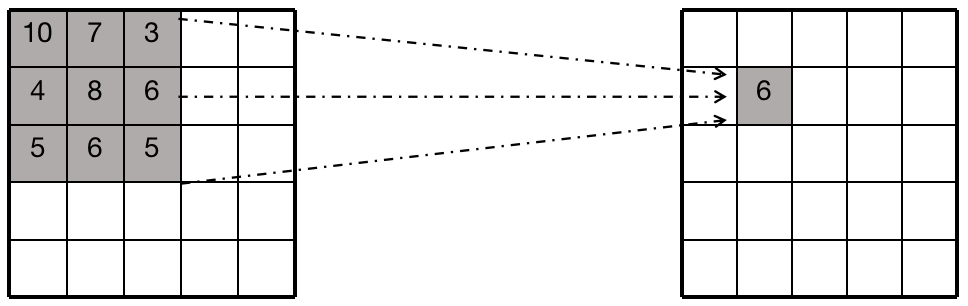
\includegraphics[width=0.45\textwidth]{Figures/cnn_conv_1.png}
    %\caption{fig1}
    }
    \quad
    \subfigure[欧式空间(图像)上的卷积2.]{
    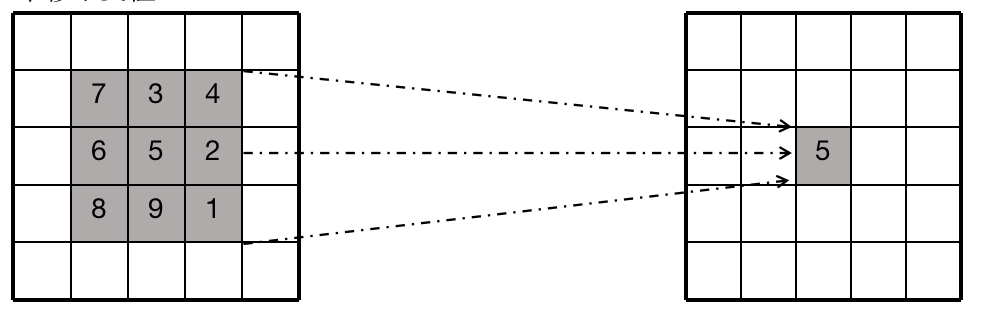
\includegraphics[width=0.45\textwidth]{Figures/cnn_conv_2.png}
    }
    \quad
    \subfigure[局部化的图卷积1.]{
    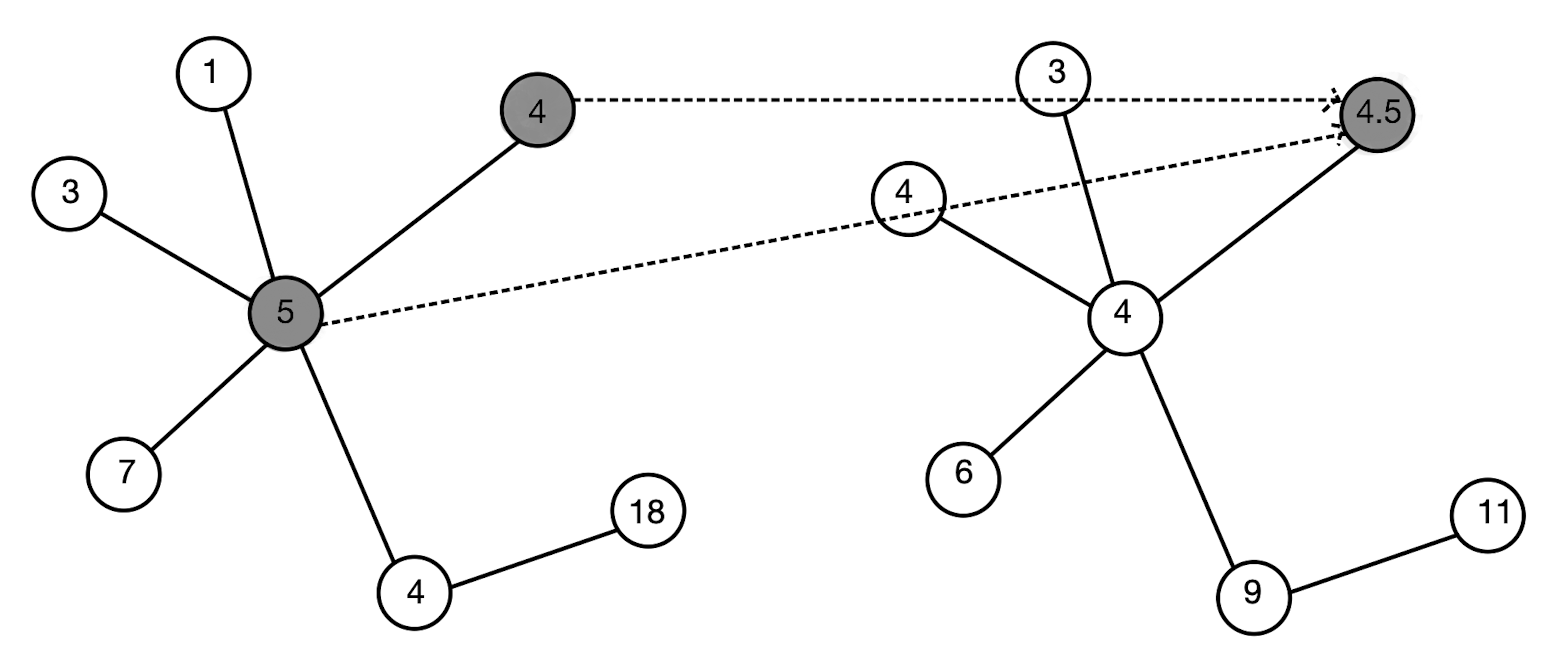
\includegraphics[width=0.45\textwidth]{Figures/graph_conv_1.png}
    }
    \quad
    \subfigure[局部化的图卷积2.]{
    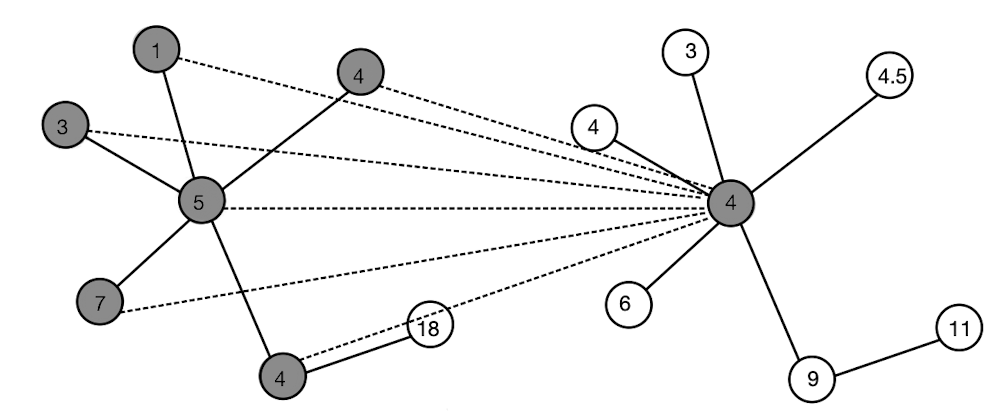
\includegraphics[width=0.45\textwidth]{Figures/graph_conv_2.png}
    }
    \caption{图像上的卷积与图卷积。第一排的两张图片展示了CNNs中的卷积。
    可以看到(a)和(b)中卷积算子(灰色部分)规模相同,且天然具有聚合邻居的作用,
    满足了平移不变性和局部性;第二排的两张图片则展示了局部化的图卷积,
    显然在不同位置的卷积算子规模不同,导致这样的图卷积不满足平移不变性。}
    \label{fig:compare_convs}
  \end{figure}

  \textbf{(1)卷积定理}:
  信号卷积的傅立叶变换等价于信号的傅立叶变换的乘积:
  \begin{equation} \label{conv_law_1}
    F(f \times g) = F(f) \centerdot F(g)
  \end{equation}
  由此可得:
  \begin{equation} \label{conv_law_2}
    f \times g = F^{-1}(F(f) \centerdot F(g))
  \end{equation}
  其中$F(\centerdot)$为图上的傅立叶变换,
  $F^{-1}(\centerdot)$则表示图上的傅立叶逆变换。

  \textbf{(2)图上的傅立叶变换、傅立叶逆变换}:
  根据谱图理论,图上的傅立叶变换是以归一化的图的拉普拉斯矩阵$\mathbf{L}$的特征向量为基底的变换,
  其中 $\mathbf{L}= \mathbf{I}_n - 
  \mathbf{D}^{-\frac{1}{2}}\mathbf{A}\mathbf{D}^{-\frac{1}{2}}$。
  对$\mathbf{L}$进行特征分解(或称谱分解)有:
  \begin{equation} \label{eigen_decomp_L}
    \mathbf{L} = \mathbf{U}\Lambda\mathbf{U}^{T}
  \end{equation}
  其中,$\mathbf{U}$为特征向量组成的矩阵,每一列为一个特征向量$\mathnormal{u_i}$;
  $\Lambda$则为以特征值为作为对角线处值的对角矩阵。
  在此基础上,傅立叶变换将图上的原始信号$x$转换为谱域下的信号$\hat{x}$的过程表达为:
  \begin{equation} \label{fourier_trans}
    \hat{x} = {\mathbf{U}}^{T}x
  \end{equation}
  同时可以得到,傅立叶逆变换将图上的谱域信号$\hat{x}$转换为原始信号$x$的过程表达为:
  \begin{equation} \label{reverse_fourier_trans}
    x = \mathbf{U}\hat{x} 
  \end{equation}

  \textbf{(3)基于卷积定理的图卷积}:
  至此,我们可以利用卷积定理定义图卷为:
  \begin{equation} \label{graph_conv_raw}
    \mathnormal{x}{\ast}_{\mathnormal{G}}\mathnormal{y} = 
    \mathbf{U}((\mathbf{U}^T\mathnormal{x}) \circ (\mathbf{U}^T\mathnormal{y}))
  \end{equation}
  不妨把公式\ref*{graph_conv_raw}中的$\mathnormal{x}$作为输入信号,
  $\mathbf{U}^T\mathnormal{y}$作为卷积核。
  为方便之后模型的公式化表达,我们对卷积核进行参数化,具体做法为:
  把向量$\mathbf{U}^T\mathnormal{x}$和向量$\mathbf{U}^T\mathnormal{y}$
  的哈达玛积转化为对角矩阵$\mathnormal{g}_\theta$和向量$\mathbf{U}^T\mathnormal{x}$的乘积,
  则公式\ref*{graph_conv_raw}转化为:
  \begin{equation} \label{graph_conv_gtheta}
    GConv(\mathnormal{x}) = 
    \mathbf{U}\mathnormal{g}_\theta\mathbf{U}^T\mathnormal{x} 
  \end{equation}
  其中,$GConv(.)$表示图卷积算子,$\mathnormal{g}_\theta$表示新的、经过参数化表示的卷积核。
  % 把公式\ref*{graph_conv_raw}中的信号$\mathnormal{x}$看作我们的输入信号,
  % 把信号$\mathnormal{y}$看作

  \textbf{(4)利用切比雪夫多项式参数化卷积核}:
  为了避免对图的拉普拉斯矩阵$\mathbf{L}$进行特征分解时带来的巨大计算量,
  ChebyNet\textsuperscript{\cite{ChebyNet}}利用正则化的特征值矩阵$\hat{\Lambda}$的切比雪夫多项式
  继续参数化卷积核$\mathnormal{g}_\theta$并
  结合公式\ref*{eigen_decomp_L}有如下推导:
  \begin{align} \label{cheby_conv}
      GConv(\mathnormal{x}) &= \mathbf{U} \mathnormal{g}_\theta \mathbf{U}^T \mathnormal{x} \notag\\
      &= \mathbf{U} (\sum^{K}_{k=0}\theta_k\mathnormal{T}_k(\hat{\Lambda}) ) 
          \mathbf{U}^T \mathnormal{x}\notag \\
      &=  (\sum^{K}_{k=0}\theta_k\mathnormal{T}_k(\hat{\mathnormal{L}}) ) 
           \mathnormal{x} \notag \\ 
  \end{align}
  其中,$\theta_k$是需要学习的网络参数,$\mathnormal{T}_k(.)$表示
  切比雪夫多项式的第$k$项,
  $\hat{\Lambda} = \frac{2\Lambda}{\lambda_{max}} - \mathbf{I}_n$,
  $\hat{\mathbf{L}} = \frac{2\mathbf{L}}{\lambda_{max}} - \mathbf{I}_n$。
  
  \textbf{(5)对ChebyNet的一阶近似}:
  公式\ref*{cheby_conv}中的$K$表示卷积算子涵盖的范围为$K$跳,
  即每个节点会同$K$跳内的节点做卷积。
  Kipf等人基于ChebyNet的参数化方法卷积算子,
  构建了ChebyNet的一阶近似,即一阶梯图卷积神经网络(GCN)\textsuperscript{\cite{kipfGCN}},具体方法见下。

  首先约束$K = 1$,且$\lambda_{max} = 2$,则可以得到:
  \begin{equation} \label{gcn_conv_1}
    GConv(\mathnormal{x}) = {\theta_0}'\mathnormal{x} + {\theta_1}'(\mathbf{L}-\mathbf{I}_n)\mathnormal{x}
    = {\theta_0}'\mathnormal{x} - {\theta_1}'\mathbf{D}^{-\frac{1}{2}}\mathbf{A}\mathbf{D}^{-\frac{1}{2}}
  \end{equation}

  为了减少计算量并防止可能的过拟合,我们令$\theta = {\theta_0}' = -{\theta_1}'$
  于是公式\ref*{gcn_conv_1}化简为:
  \begin{equation} \label{gcn_conv_2}
    GConv(\mathnormal{x}) = \theta(\mathbf{I}_n + 
    \mathbf{D}^{-\frac{1}{2}}\mathbf{A}\mathbf{D}^{-\frac{1}{2}})\mathnormal{x}
  \end{equation}

  此外,为了维持数值稳定,防止出现梯度爆炸和梯度消失的问题,我们对公式\ref*{gcn_conv_2}
  作出如下正则化:
  \begin{equation} \label{gcn_conv_3}
    \mathbf{I}_n + \mathbf{D}^{-\frac{1}{2}}\mathbf{A}\mathbf{D}^{-\frac{1}{2}} 
    \rightarrow
    \tilde{\mathbf{D}}^{-\frac{1}{2}} \tilde{\mathbf{A}} \tilde{\mathbf{D}}^{-\frac{1}{2}} 
  \end{equation}
  其中$\tilde{\mathbf{A}} = \mathbf{I}_n + \mathbf{A}$, 
  $\tilde{\mathbf{D}}_{ii} = \sum_j\tilde{\mathbf{A}}_{ij}$

  最终我们得到GCN\textsuperscript{\cite{kipfGCN}}中的卷积算子为:
  \begin{equation} \label{gcn_conv_4}
    GConv(\mathnormal{x}) = 
    (\tilde{\mathbf{D}}^{-\frac{1}{2}} \tilde{\mathbf{A}} \tilde{\mathbf{D}}^{-\frac{1}{2}})
    \mathnormal{x}
    \theta
  \end{equation}
  将卷积算子延伸至多通道情况下,可以得到GCN在第$m$层的前向传播公式为:
  \begin{equation} \label{gcn_forward}
    \mathbf{X}^{m+1} = \sigma(
      \tilde{\mathbf{D}}^{-\frac{1}{2}} \tilde{\mathbf{A}} \tilde{\mathbf{D}}^{-\frac{1}{2}}
      \mathbf{X}^{m}\Theta^{m}
      )
  \end{equation}
  其中,$\sigma$为层间的激活函数($ReLU, sigmoid, tanh$等),$ \tilde{\mathbf{D}}^{-\frac{1}{2}} \tilde{\mathbf{A}} \tilde{\mathbf{D}}^{-\frac{1}{2}}$
  是非参数化的一阶近似卷积核,$\Theta^{m}$则为需要学习的第$m$层的网络参数。GCN的模型结构如下图所示。
  \begin{figure}[htbp]
    \centering
    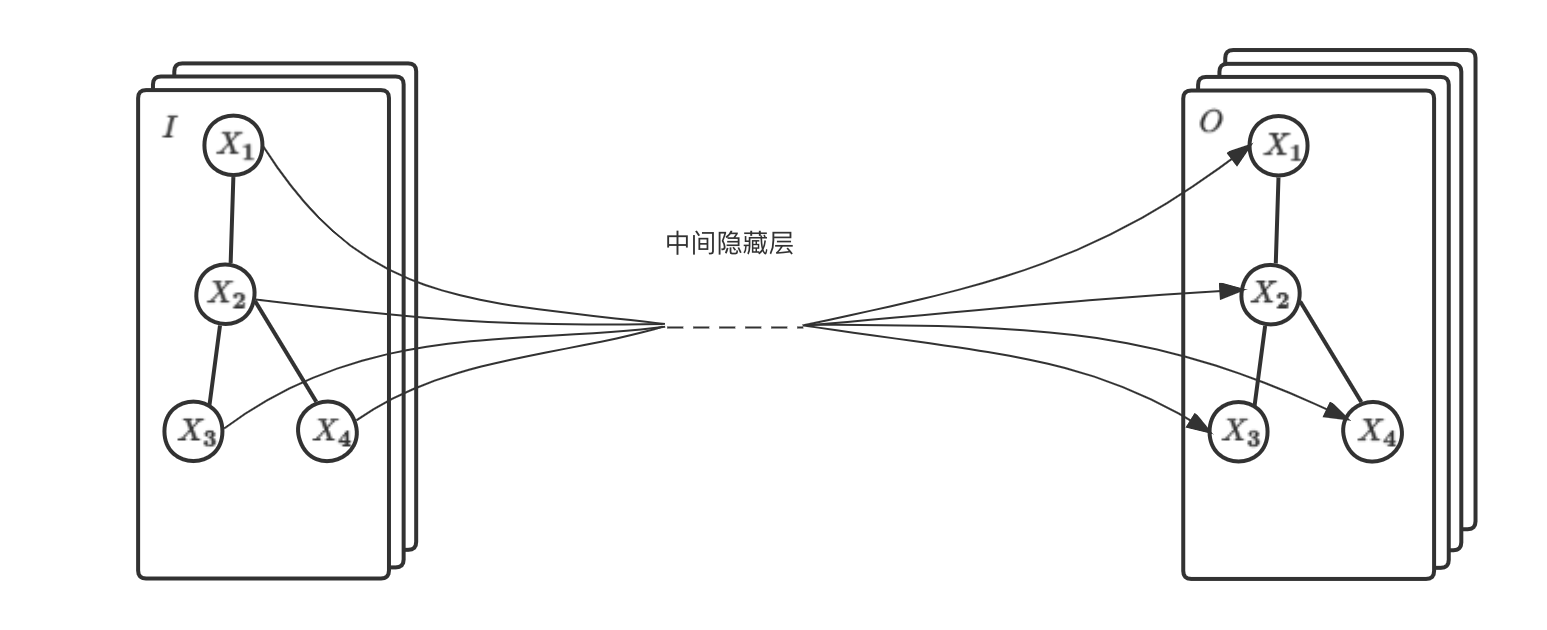
\includegraphics[width=0.8\textwidth]{Figures/GCN-model.png}
    \caption{GCN模型结构图例;$I$表示输入通道数目即输入的图中每个节点的特征向量维度,$O$则表示输出通道数;
    输入的图结构在所有层中是共享的,因此图卷积核在各层也是共享的;}
    \label{pic:GCN-model}
  \end{figure}
  
  \section{循环神经网络} \label{sec:B2}
      % RNN部分的符号表
      \begin{center}
        \tablecaption{本节符号表}
        \begin{tabular}{ll}
          \toprule
          符号 & 含义\\ 
          \midrule
          $\mathbf{x}$ & 观察到的序列 \\
          $x_i$ & 序列$\mathbf{x}$中第$i$项 \\
          $p(x_i | x_1,x_2,...,x_{i-1})$ & 序列中$x_i$出现的概率(条件概率)\\
          $f(x_1, x_2, x_3,...,x_{i-1})$ & 泛指序列模型对序列中第$i$项之前的历史信息的建模 \\
          $h_i$ & 潜变量;潜变量模型中对序列中第$i$项之前的历史信息的建模 \\
          $y_i$ & 序列模型对$x_i$的预测 \\
          $F(.)$ & 由$h_{i-1}$和$x_i$到$h_i$的映射 \\
          $\Phi$ & 泛指各种非线性的激活函数 \\
          $\sigma$ & 非线性激活函数$ReLU$ \\
          $W_{**}, b_{*}$ & 仿射变换中的权重和偏移 \\ 
          $\circ$ & 哈达玛积 \\
          \bottomrule
        \end{tabular}
      \end{center}

      上节我们详细地介绍了图卷积和欧式空间卷积的不同之处和定义的难点,
      并讲述了本文关注的图卷积神经网络GCN中一阶近似图卷积(公式\ref{gcn_conv_4})的理论
      推导过程。本节我们将详细阐明EvolveGCN中用于驱动参数训练的部分--循环神经网络。

      \textbf{2.2.1 序列模型和潜变量的引入}

      现实生活中存在着具有时序结构的数据,比如按照单词顺序排列而成的句子、
      按照时间顺序呈现的视频或者音频、
      按照时间顺序排列的银行交易数据等等。
      序列模型就是针对这样的数据设计的用来接受某一序列作为输入,
      并预测该序列后续的模型。
      循环神经网络便是当今使用最为广泛、效果最好的的序列模型。

      序列模型同非序列模型的本质区别在于,
      序列模型中当前的数据同先前观察到的数据是相关的。
      不妨假设我们在$\mathnormal{t}$时刻观察到数据$\mathnormal{x_t}$,
      共有$\mathnormal{T}$个时刻的数据组成序列$\mathbf{x}$,
      那么序列$\mathbf{x}$出现的概率为$\mathnormal{p(\mathbf{x})}$。
      由于$\mathnormal{x_t}$之间具有如上所述的相关性,根据条件概率公式:
      \begin{equation} \label{seq_x_prob}
        \mathnormal{p(\mathbf{x})} = 
        \mathnormal{p(x_1)\centerdot p(x_2 | x_1) \centerdot 
        p(x_3 | x_1,x_2) \centerdot ... p(x_T| x_1,...x_{T-1}) }
      \end{equation}
      上式中的某一项表示序列中某一时刻的观察值$x_t$的概率,
      对该项中的历史信息$\mathnormal{x_1,x_2,...,x_{t-1}}$建模有:
      \begin{equation} \label{xt_prob_without_ht}
        \mathnormal{p(x_t | x_1, x_2, ..., x_{t-1})} = \mathnormal{
          p(x_t | f(x_1, x_2,...,x_{t-1}))
        }
      \end{equation}
      其中的$f(.)$表示对过去信息的建模。
      潜变量模型通过引入潜变量$h_t$来表示$t$时刻之前的历史信息$f(x_1, x_2,...,x_{t-1})$:
      \begin{equation} \label{xt_prob_with_ht}
        \mathnormal{p(x_t | x_1, x_2, ..., x_{t-1})} = \mathnormal{
          p(x_t | h_t)
        }
      \end{equation}
      因此基于潜变量的序列模型(循环神经网络)可以描述为:
      接受一个序列$\mathbf{x} ={x_1, x_2, x_3,..., x_T}$作为输入,
      模型运行至$t$时刻时,
      通过映射$F(.)$将上一个时刻的潜变量$h_{t-1}$和当前的输入信息$x_t$映射到$t$时刻的潜变量$h_t$,
      然后根据$h_t$预测$t$时刻的结果$y_t = p(x_t | h_t)$。
      其中,组合上一时刻的潜变量和当前时刻的信息的映射$F(.)$
      成为了不同类型循环神经网络的主要区别。
      接下来我们将针对这方面的不同来说明基础的RNN--Vanilla RNN以及GUR和LSTM的原理。

      % 插入RNN的广义示意图
      \begin{figure}[htbp]
        \centering
        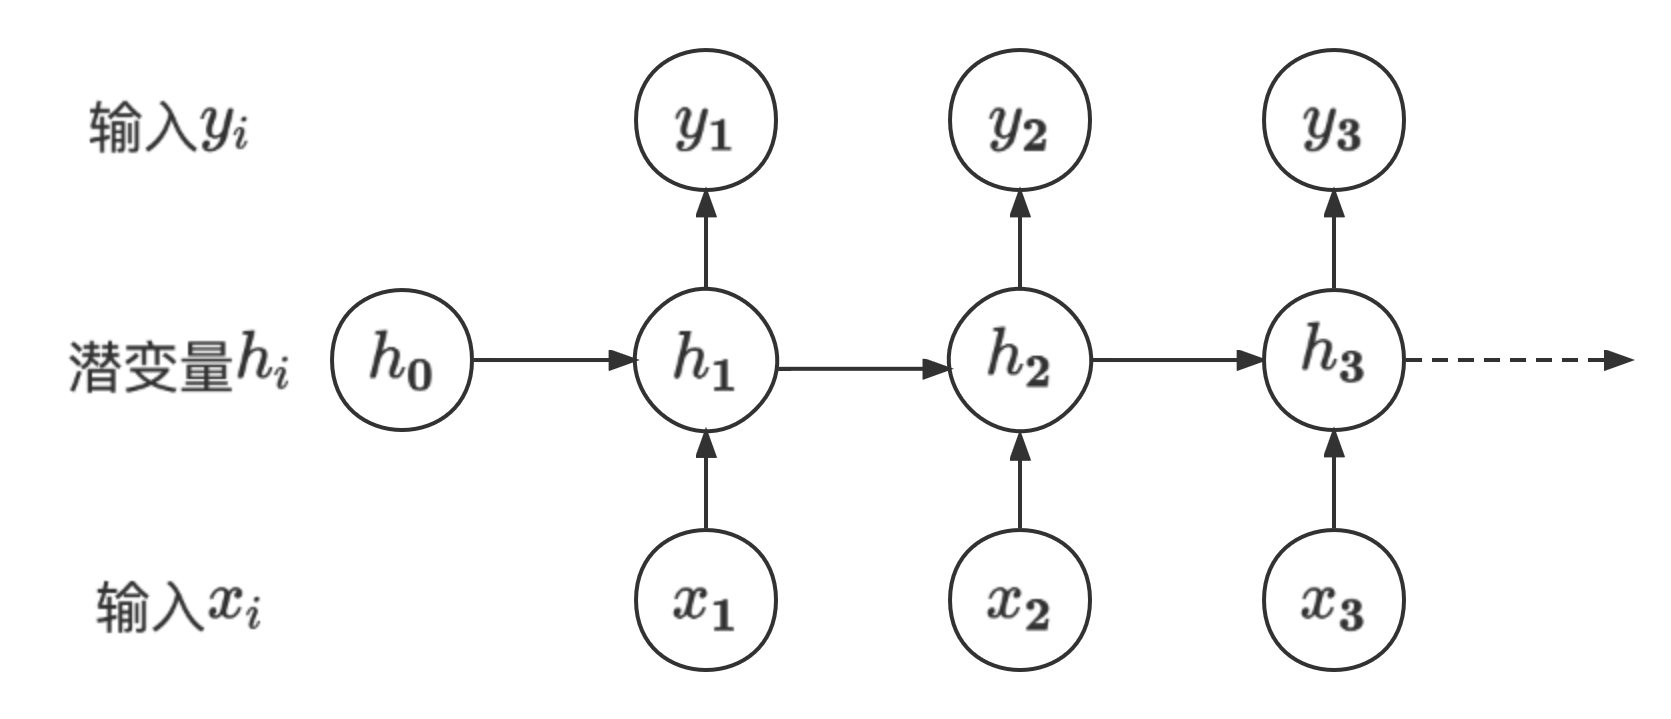
\includegraphics[width=0.8\textwidth]{Figures/RNNs.png}
        \caption{各种RNNs宏观基本结构}
        \label{pic:RNNs}
      \end{figure}
      
      \textbf{2.2.2 Vanilla RNN}

      Vanilla RNN是最简单明了的RNN,
      它通过对$h_{t-1}$和$x_{t}$做线性变换得到潜变量$h_t$。
      \begin{equation} \label{va_rnn_hidden}
        \mathnormal{h_t} = \Phi(\mathnormal{W_{hh}}\mathnormal{h_{t-1}} + 
        \mathnormal{W_{hx}}\mathnormal{x_{t}} + \mathnormal{b_h})
      \end{equation}
      同样的,输入$y_t = p(x_t | h_t)$也是简单地对$h_t$进行线性变化得到。
      \begin{equation}
        \mathnormal{y_t} = \Phi(W_{hy}h_t + b_y)
      \end{equation}
    其中,$\Phi$表示非线性的激活函数,$W_{**}$表示权重,$b_*$则表示偏移。

      \textbf{2.2.3 LSTM和GRU}

      相比Vanilla RNN,LSTM和GRU则复杂得多。它们通过引入若干门和候选状态对历史信息进行更新、遗忘和筛选,
      从而使得新的潜变量$h_t$具有更为精细、准确的历史信息。其详细流程分述如下。

      \textbf{(1)LSTM}:长短时记忆(Long Short Term Memory)又称LSTM,
    它在Vanilla RNN的基础上引入了和隐变量形状相同的记忆单元$C_t$来记录额外的信息,
    并通过引入输入门$I_t$, 遗忘门$F_t$, 输出门$O_t$来控制记忆单元筛选历史信息。
    各个门的计算方法为:
    \begin{align}
      I_t &= \sigma(x_t W_{xi} + h_{t-1}W_{hi} + b_i)  \\
      F_t &= \sigma(x_t W_{xf} + h_{t-1}W_{hf} + b_f)  \\
      O_t &= \sigma(x_t W_{xo} + h_{t-1}W_{ho} + b_o)  \\
      \notag
    \end{align} 
    其中,$\sigma$是非线性激活函数$ReLU$,输入门$I_t$控制哪些信息输入到记忆单元$C_t$,
    输出门$O_t$负责配合记忆单元$C_t$得到$h_t$,
    遗忘门$F_t$则负责重置$C_t$中的内容。
    此外,LSTM还包括候选记忆单元$\tilde{C_t}$。
    它同三个门的计算方式类似,只是采用了$tanh$作为激活函数,其计算公式为:
    \begin{equation}
      \tilde{C_t} = tanh(x_t W_{xc} + h_{t-1} W_{hc} + b_c)
    \end{equation}
    有了上述三个门以及候选记忆单元,LSTM便可以得到新的记忆单元$C_t$和隐变量$h_t$。
    某个步骤内完整的LSTM流程见图\ref{pic:LSTM}。
    \begin{align}
      C_t = F_t\circ C_{t-1} + I_t \circ \tilde{C_t} \\
      h_t = O_t \circ tanh(C_t)
    \end{align}
      \begin{figure}[htbp]
        \centering
        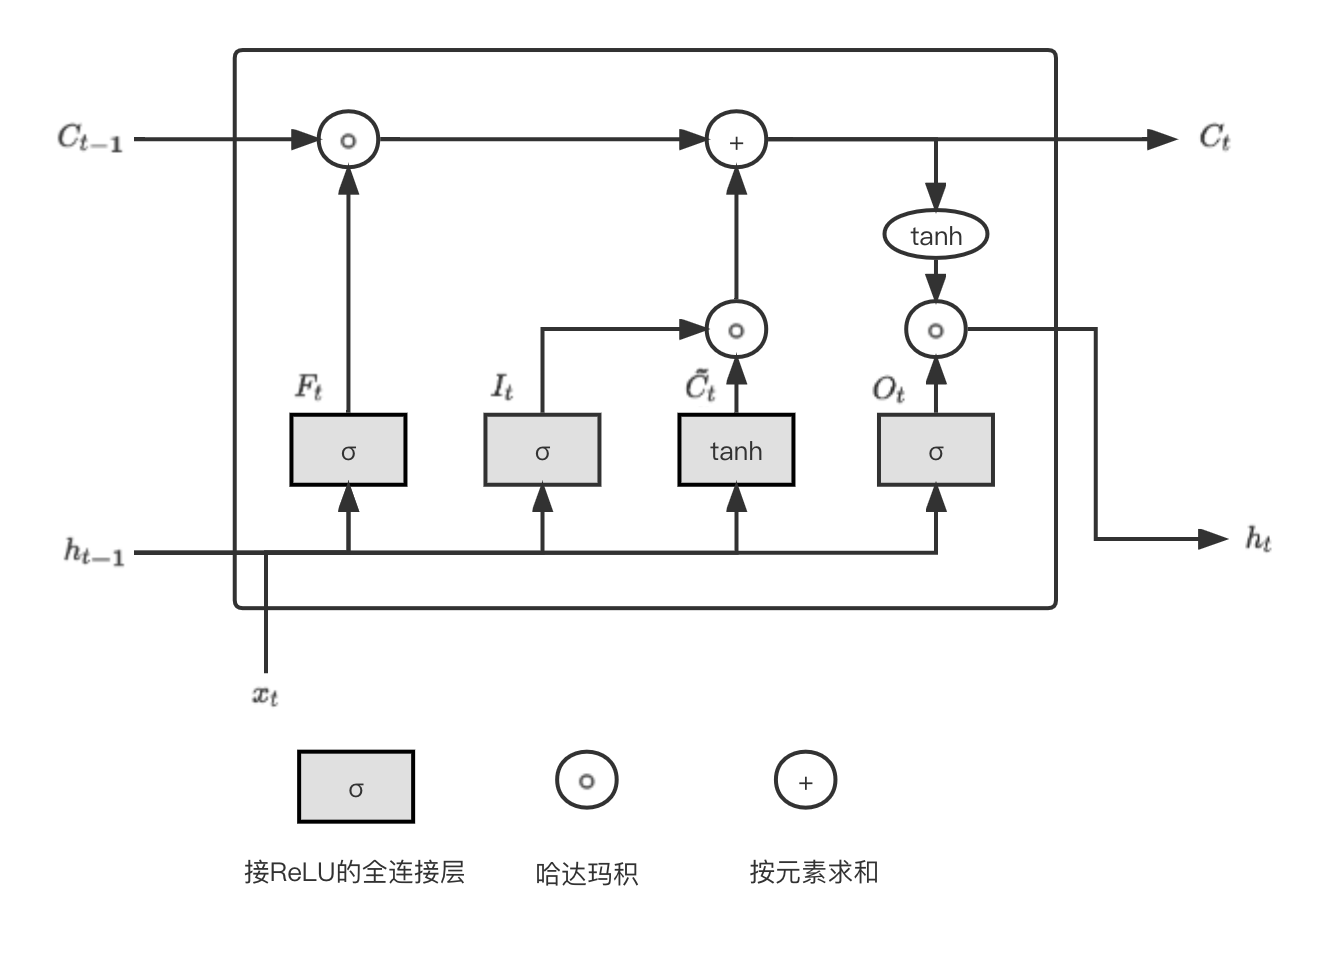
\includegraphics[width=0.8\textwidth]{Figures/LSTM.png}
        \caption{LSTM流程图}
        \label{pic:LSTM}
      \end{figure}

      \textbf{(2)GRU}: 门控循环单元(Gated Recurrent Unit) 又称GRU,它同LSTM类似,
      通过引入候选潜变量$\tilde{h_t}$来记录额外的信息,
      并通过重制门$R_t$和更新门$Z_t$来控制候选潜变量筛选历史信息。重制门和更新门的计算方式为:
      \begin{align}
        R_t = \sigma(x_t W_{xr} + h_{t-1} W_{hr} + b_r) \\
        Z_t = \sigma(x_t W_{xz} + h_{t-1} W_{hz} + b_z) 
      \end{align}
      和LSTM中的候选记忆单元类似,GRU具有候选潜变量$\tilde{h_t}$,
      \begin{equation} \label{gru_cand_ht}
        \tilde{h_t} = tanh(x_t W_{xh} + (R_t \circ h_{t-1})W_{hh} + b_h)
      \end{equation}
      其中的$R_t \circ h_{t-1}$ 部分实际上是进行了对历史信息的筛选:
      当$R_t$接近1时, 公式\ref{gru_cand_ht}等价于公式\ref{va_rnn_hidden},
      GRU将近似退化为Vanilla RNN;
      而当$R_t$接近0时,$\tilde{h_t}$则完全不考虑历史信息,只考虑当前输入$x_t$。
      根据候选潜变量$\tilde{h_t}$以及更新门,我们可以得到新的潜变量如下:
      \begin{equation} \label{gru_ht}
        h_t = Z_t \circ h_{t-1} + (1-Z_t)\circ \tilde{h_t}
      \end{equation}
      当更新门$Z_t$接近1时,模型则保留原有状态$h_{t-1}$;
      而当其接近0时,模型则倾向选择候选潜变量$\tilde{h_t}$作为新的潜变量$h_t$。
      某个步骤内完整的GRU流程见图\ref{pic:gru}。
      \begin{figure}[htbp]
      \centering
      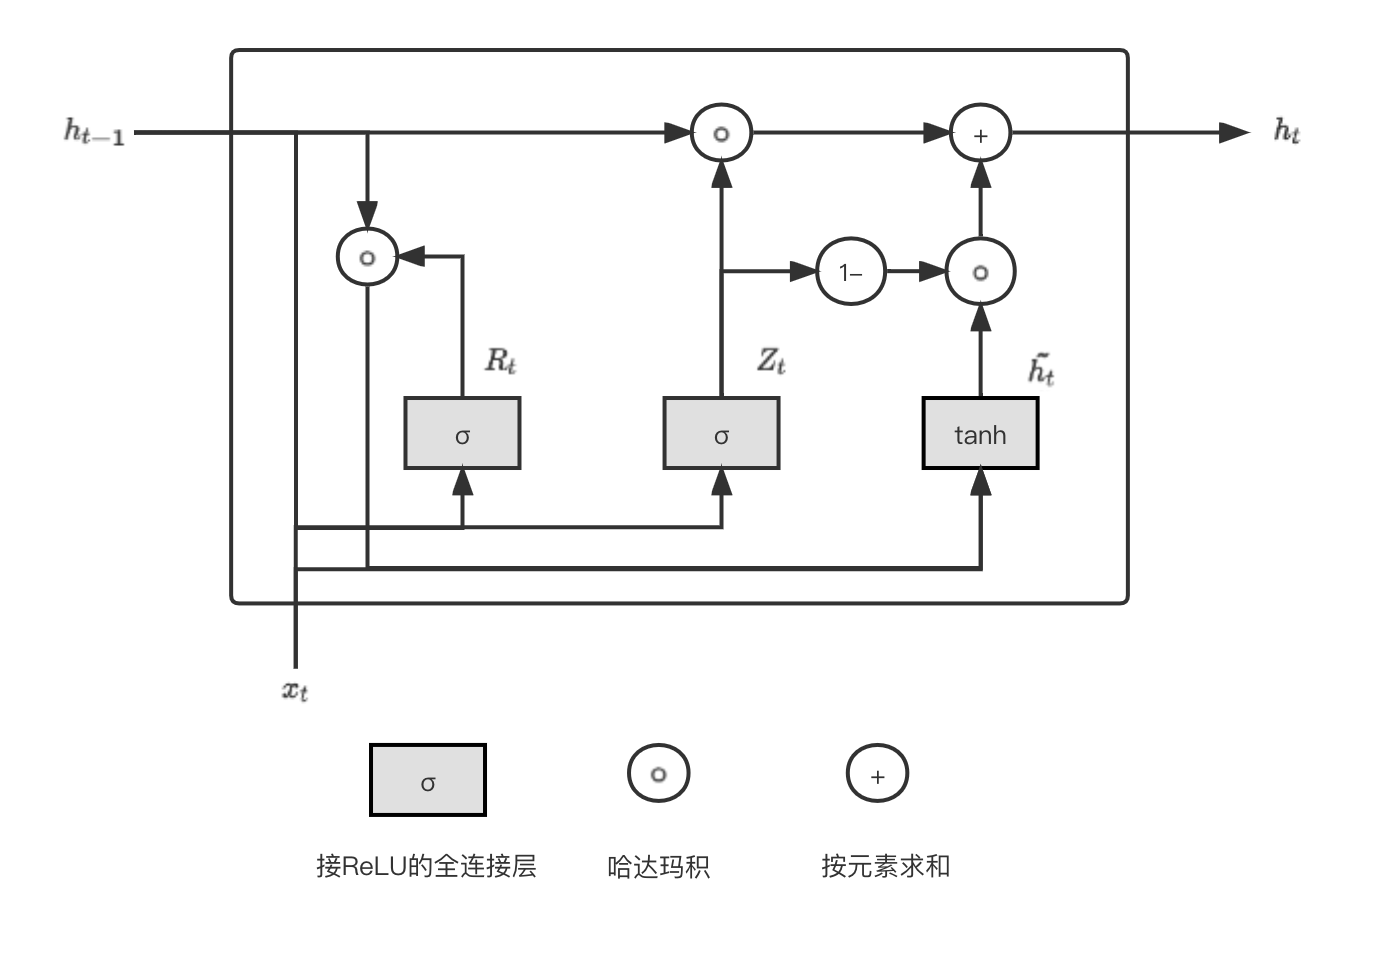
\includegraphics[width=0.8\textwidth]{Figures/GRU.png}
      \caption{GRU流程图}
      \label{pic:gru}
    \end{figure}
  
  \section{半监督学习} \label{sec:B3}

  机器学习方法可以按照样本的标记情况分为三类:所有样本数据都无标签的无监督学习、所有样本数据都有标签的监督学习以及
  本节的主要讨论对象、仅部分样本数据有标签的半监督学习。

  无监督学习的样本数据不具有标签,因此只能从样本数据的分布和它们之间的关系着手,
  将样本划分至不同簇(聚类)或者是给出高维样本的低维表示(降维)。
  典型的无监督算法有:聚类算法中的K均值(K-means)
  和降维算法中的主成分分析(Principle Component Analysis)等。

  监督学习则是机器学习领域中发展最成熟、最为迅速的一类算法,
  它利用有标签的样本数据训练出从样本数据到标签的映射,
  从而对模型未见过的样本数据的标签进行预测。
  典型的监督学习算法有:线性回归(Linear Regression)、
  线性判别分析(Linear Discriminative Analysis)、
  Logistic回归(Logisitic Regression)、
  支持向量机(Support Vector Machine)、
  朴素贝叶斯(Naive Bayes)、决策树(Decision Tree)
  以及多层感知机(Multi-Layer Perceptron)等。

  实际问题中,海量样本数据是容易获得的,
  然而由于样本数据的标记工作专业性要求高、工作量巨大,
  完成对这些海量样本数据的标记需要消耗大量时间、人力等资源。
  因此有标签的样本数据和无标签的样本数据往往是同时存在的,
  而且无标签样本数据常占很高的比例。
  为了更充分地利用样本数据、减少数据和资源的浪费并提高模型的效果,
  人们尝试把大量没有标签的样本数据同少数有标签的样本数据一起
  注入到模型的训练过程中,半监督学习方法由此应运而生。
  结合\ref{chpt:A}\ref{sec:B2}对问题的描述,
  本文拟完成的反洗钱任务的样本数据表现为小部分样本数据有标签、大部分样本数据无标签,
  因此应该采用半监督学习的模型。
  下面介绍\ref{chpt:B}\ref{sec:B1}中的GCN是如何进行半监督学习的。

  从公式\ref{gcn_conv_4}可以看出GCN的卷积核
  $\tilde{\mathbf{D}}^{-\frac{1}{2}} \tilde{\mathbf{A}} \tilde{\mathbf{D}}^{-\frac{1}{2}} \in \mathbb{R}^{n*n}$是非参数化的,
  即它只取决于整张图的拓扑结构(邻接矩阵)。
  这样的特点使得我们能够利用所有样本数据得到全局共享的卷积核,
  接着对所有样本的特征映射$\mathbf{X} \in \mathbb{R}^{n*d}$依次进行
  卷积操作、仿射变换和非线性激活操作。
  至此GCN完成了一次前向传播($Forward$)而没有关心样本数据的标记情况。
  GCN完成前向传播转而进行后向传播($Backward$)时则需要考虑样本数据的标记情况:
  只利用带有标签的样本对应的输出层特征映射和标记情况进行损失的计算和网络参数的更新。综上所述,
  GCN利用全体样本数据的邻接矩阵和特征映射完成了前向传播,
  而利用带有标签的样本数据完成了后向传播从而实现半监督学习,其训练过程的伪代码如下:

    \begin{algorithm}[htbp]
      \caption{GCN训练过程伪代码}
      \label{alg:GCN-process}
      \hspace*{0.04in}{\bf Inputs:}\\
      模型层数$m$\\
      模型$model$\\
      所有样本形成的邻接矩阵$\mathbf{A} \in \mathbb{R}^{n*n}$\\
      所有样本的特征映射$\mathbf{X}^{0} \in \mathbb{R}^{n*d}$\\
      第一层网络参数$\Theta^{0}$\\
      损失函数$\mathbf{L}$\\
      所有样本的标记情况$Labels \in \mathbb{R}^{n}$\\
      带有标签的训练样本的筛选器$train\_mask \in \mathbb{R}^{n_{train}}$ \\
      \begin{algorithmic}[1]
        \State 由$\mathbf{A}$得到全局共享的卷积核
        $\tilde{\mathbf{D}}^{-\frac{1}{2}} 
        \tilde{\mathbf{A}} 
        \tilde{\mathbf{D}}^{-\frac{1}{2}}$ \\
        \\
        \% $\textbf{Forward:} $
        \For{$i \ in \ range(m)$ }
          \State 
          $\mathbf{X}^{i+1} = \sigma(
            \tilde{\mathbf{D}}^{-\frac{1}{2}} \tilde{\mathbf{A}} \tilde{\mathbf{D}}^{-\frac{1}{2}}
            \mathbf{X}^{i}\Theta^{i}
            )$
        \EndFor
        \\
        \State
        \% $\textbf{Backward:}$\\
        输出的特征映射:$\mathbf{X}^{m} \in \mathbb{R}^{n*{d^m}}$ \\
        筛选出带有标签的训练样本的特征映射: $\mathbf{X}^{m}_{train} = \mathbf{X}^{m}[train\_mask]$ \\
        筛选出带有标签的训练样本的标记情况: $Labels_{train} = Labels[train\_mask]$ \\ 
        利用带有标签的训练样本计算损失:$Loss = \mathbf{L}(\mathbf{X}^{m}_{train}, Labels_{train})$ \\

        $Loss.backward()$ \\
        $Update(model)$
      \end{algorithmic}
    \end{algorithm}

  \section{本章小结} \label{sec:B4}
  本章对EvolveGCN所需的理论基础进行了介绍。
  详细地说明了图卷积神经网络GCN和循环神经网络GRU、LSTM的原理,
  并介绍了GCN进行半监督学习的运行。
  接下的一章我们将以此为基础,详细介绍EvolveGCN的模型原理。

\chapter{模型原理} \label{chpt:C}
  \section{数据存储和处理方式}
  \begin{enumerate}
    \item 按时间划分;多重边的合并;有向图转为无向图; 稀疏矩阵的存储;
  \end{enumerate}
  
  \section{RNN驱动训练}
  上图和解析;
    
  \section{模型评价机制}
  分类别的precision、recall和f1;着重关注黑标节点的precision

\chapter{实验} \label{chpt:D}
  \section{实验条件}
  \section{实验流程}
  \section{实验结果}

\chapter{讨论和总结} \label{chpt:E}
  \begin{enumerate}
    \item 优点:适用于动态图,把时序信息融合在训练过程中
    \item 缺点:基于GCN,使得其必然是Transductive的,
    且对内存有极高要求
  \end{enumerate}


% -*- coding: utf-8 -*-
% \chapter{参考文献}
\zihaowu
% %\renewcommand{\bibname}{参考文献}
% %\def\bibrangedash{ $\sim$ }
% %\printbibliography
% \def\bibrangedash{ $\sim$ }
% \printbibliography [ category = cited]
\renewcommand\bibname{参考文献}
% \begin{thebibliography}{99}  
%     \bibitem{kipf2016semi}Kipf, T. \& Welling, M. Semi-supervised classification with graph convolutional networks. {\em ArXiv Preprint ArXiv:1609.02907}. (2016)
%     \bibitem{ref1}Zheng L, Wang S, Tian L, et al., Query-adaptive late fusion for image search and person re-identification, Proceedings of the IEEE Conference on Computer Vision and Pattern Recognition, 2015: 1741-1750.  
%     \bibitem{ref2}Arandjelović R, Zisserman A, Three things everyone should know to improve object retrieval, Computer Vision and Pattern Recognition (CVPR), 2012 IEEE Conference on, IEEE, 2012: 2911-2918.  
%     \bibitem{ref3}Lowe D G. Distinctive image features from scale-invariant keypoints, International journal of computer vision, 2004, 60(2): 91-110.  
%     \bibitem{ref4}Philbin J, Chum O, Isard M, et al. Lost in quantization: Improving particular object retrieval in large scale image databases, Computer Vision and Pattern Recognition, 2008. CVPR 2008, IEEE Conference on, IEEE, 2008: 1-8.  
% \end{thebibliography}
\printbibliography
\end{spacing}
% -*- coding: utf-8 -*-

\begin{zhixie}
乌飞兔走,白驹过隙;时光荏苒,岁月如歌。

转眼间我和南开的故事就要画上句号了,
四年时光里有过入学前的憧憬和激动,也有过重复中的枯燥单调和乏味;
有过输掉第一场篮球比赛的落寞和不甘,也有过乘胜追击时的酣畅淋漓;
有过第一个学期的迷茫和困惑,也有过保研成功、金榜提名的欣慰和满足;
有过收到‘好人卡’的苦涩和自卑,也有了一段平淡幸福,充满希望的感情;
有过深夜的酒,也有过清晨的书。
有过酸甜,有过苦辣,平凡而又充实。

感谢南开大学给了我更高的平台、更广阔的视野;
感谢软件学院各位老师们的悉心教导,让我进入到蓬勃发展的计算机领域;
感谢女友的一路支持、鼓励和陪伴;
感谢各位球友一起挥汗如雨,享受运动的快乐;
感谢君儿、轩儿、俊宇和‘智商’。



\end{zhixie}
\include{appendices}
% -*- coding: utf-8 -*-


\chapter*{个人简历}

\noindent 基本信息:\\

 姓名:~王子旭
 
 性别:~男 

 出生日期:~2000年03月23日

 通信地址:~南开大学软件学院/中国科学院计算技术研究所

 电  话:15631008979

 E-mail:~1813033@mail.nankai.edu.cn \\ \\
\\
教育背景:\\  

2018.09-2022.07 \quad 南开大学\quad 软件学院\quad\quad 软件工程\quad\quad 学士 \\ 
%2012年9月-2016年7月\quad 南开大学\quad 某某学院\quad\quad\quad\quad 某某学\quad\quad 硕士 \\
\\
%硕士期间发表的学术论文:\\


\end{document}

